\textit{``We should interrogate the architecture of cyberspace as we interrogate the code of Congress.''}
– Lawrence Lessig 
\chapter{Introduction}
The past three years have seen a small profusion of websites, perhaps as many as 80, spring up to capitalize on the high interest that mug shot photos generate online.^{\href{#endnotes}{1}} Mug shots are public record, artifacts of an arrest, and these websites collect, organize, and optimize the photos so that they're found more easily online. Proponents of such sites argue that the public has a right to know if their neighbor, romantic date, or colleague has an arrest record. Still, mug shots are not proof of conviction; they don't signal guilt. 

Having one online is likely to result in a reputational blemish; having that photo ranked as the first result when someone searches for your name on Google turns that blemish into a garish reputational wound, festering in facile accessibility. Some of these websites are exploiting this, charging people to remove their photo from the site so that it doesn't appear in online searches. It's reputational blackmail. And remember, these people aren't necessarily guilty of anything. 

To crack down on the practice, states like Oregon, Georgia, and Utah have passed laws requiring these sites to take down the photos if the person's record has been cleared. Some credit card companies have stopped processing payments for the seediest of the sites. Clearly both legal and market forces can help curtail this activity, but there's another way to deal with the issue too: algorithms. Indeed, Google recently launched updates to its ranking algorithm that down-weight results from mug shot websites, basically treating them more as spam than as legitimate information sources.^{\href{#endnotes}{2}} With a single knock of the algorithmic gavel, Google declared such sites illegitimate. 

At the turn of the millennium, 14 years ago, Lawrence Lessig taught us that ``code is law''—that the architecture of systems, and the code and algorithms that run them, can be powerful influences on liberty.^{\href{#endnotes}{3}}We're living in a world now where algorithms adjudicate more and more consequential decisions in our lives. It's not just search engines either; it's everything from online review systems to educational evaluations, the operation of markets to how political campaigns are run, and even how social services like welfare and public safety are managed. Algorithms, driven by vast troves of data, are the new power brokers in society. 

As the mug shots example suggests, algorithmic power isn't necessarily detrimental to people; it can also act as a positive force. The intent here is not to demonize algorithms, but to recognize that they operate with biases like the rest of us.^{\href{#endnotes}{4}}And they can make mistakes. What we generally lack as a public is clarity about how algorithms exercise their power over us. With that clarity comes an increased ability to publicly debate and dialogue the merits of any particular algorithmic power. While legal codes are available for us to read, algorithmic codes are more opaque, hidden behind layers of technical complexity. How can we characterize the power that various algorithms may exert on us? And how can we better understand when algorithms might be wronging us? What should be the role of journalists in holding that power to account? 

In the next section I discuss what algorithms are and how they encode power. I then describe the idea of algorithmic accountability, first examining how algorithms problematize and sometimes stand in tension with transparency. Next, I describe how reverse engineering can provide an alternative way to characterize algorithmic power by delineating a conceptual model that captures different investigative scenarios based on reverse engineering algorithms' input-output relationships. I then provide a number of illustrative cases and methodological details on how algorithmic accountability reporting might be realized in practice. I conclude with a discussion about broader issues of human resources, legality, ethics, and transparency. 

\chapter{Algorithmic Power }
An algorithm can be defined as a series of steps undertaken in order to solve a particular problem or accomplish a defined outcome.^{\href{#endnotes}{5}}Algorithms can be carried out by people, by nature, or by machines. The way you learned to do long division in grade school or the recipe you followed last night to cook dinner are examples of people executing algorithms. You might also say that biologically governed algorithms describe how cells transcribe DNA to RNA and then produce proteins—it's an information transformation process.^{\href{#endnotes}{6}}While algorithms are everywhere around us, the focus of this paper are those algorithms that run on digital computers, since they have the most potential to scale and affect large swaths of people. 

Autonomous decision-making is the crux of algorithmic power. Algorithmic decisions can be based on rules about what should happen next in a process, given what's already happened, or on calculations over massive amounts of data. The rules themselves can be articulated directly by programmers, or be dynamic and flexible based on the data. For instance, machine-learning algorithms enable other algorithms to make smarter decisions based on learned patterns in data. Sometimes, though, the outcomes are important (or messy and uncertain) enough that a human operator makes the final decision in a process. But even in this case the algorithm is biasing the operator, by directing his or her attention to a subset of information or recommended decision. Not all of these decisions are significant of course, but some of them certainly can be. 

We can start to assess algorithmic power by thinking about the atomic decisions that algorithms make, including prioritization, classification, association, and filtering. Sometimes these decisions are chained in order to form higher-level decisions and information transformations. For instance, some set of objects might be classified and then subsequently ranked based on their classifications. Or, certain associations to an object could help classify it: Two eyes and a nose associated with a circular blob might help you determine the blob is actually a face. Another composite decision is summarization, which uses prioritization and then filtering operations to consolidate information while maintaining the interpretability of that information. Understanding the elemental decisions that algorithms make, including the compositions of those decisions, can help identify why a particular algorithm might warrant further investigation. 

\section{Prioritization }
Prioritization, ranking, or ordering serves to emphasize or bring attention to certain things at the expense of others. The city of New York uses prioritization algorithms built atop reams of data to rank buildings for fire-code inspections, essentially optimizing for the limited time of inspectors and prioritizing the buildings most likely to have violations that need immediate remediation. Seventy percent of inspections now lead to eviction orders from unsafe dwellings, up from 13 percent without using the predictive algorithm—a clear improvement in helping inspectors focus on the most troubling cases.^{\href{#endnotes}{7}}

Prioritization algorithms can make all sorts of civil services more efficient. For instance, predictive policing, the use of algorithms and analytics to optimize police attention and intervention strategies, has been shown to be an effective crime deterrent.^{\href{#endnotes}{8}}Several states are now using data and ranking algorithms to identify how much supervision a parolee requires. In Michigan, such techniques have been credited with lowering the recidivism rate by 10 percent since 2005.^{\href{#endnotes}{9}}Another burgeoning application of data and algorithms ranks potential illegal immigrants so that higher risk individuals receive more scrutiny.10 Whether it's deciding which neighborhood, parolee, or immigrant to prioritize, these algorithms are really about assigning risk and then orienting official attention aligned with that risk. When it comes to the question of justice though, we ought to ask: Is that risk being assigned fairly and with freedom from malice or discrimination? 

Embedded in every algorithm that seeks to prioritize are criteria, or metrics, which are computed and used to define the ranking through a sorting procedure. These criteria essentially embed a set of choices and value-propositions that determine what gets pushed to the top of the ranking. Unfortunately, sometimes these criteria are not public, making it difficult to understand the weight of different factors contributing to the ranking. For instance, since 2007 the New York City Department of Education has used what's known as the value-added model (VAM) to rank about 15 percent of the teachers in the city. The model's intent is to control for individual students' previous performance or special education status and compute a score indicating a teacher's contribution to students' learning. When media organizations eventually obtained the rankings and scores through a Freedom of Information Law (FOIL) request, the teacher's union argued that, ``the reports are deeply flawed, subjective measurements that were intended to be confidential.''^{\href{#endnotes}{11}}Analysis of the public data revealed that there was only a correlation of 24 percent between any given teacher's scores across different pupils or classes. This suggests the output scores are very noisy and don't precisely isolate the contribution of the teacher. What's problematic in understanding why that's the case is the lack of accessibility to the criteria that contributed to the fraught teacher rankings. What if the value-proposition of a certain criterion's use or weighting is political or otherwise biased, intentionally or not? 

\section{Classification }
Classification decisions involve categorizing a particular entity as a constituent of a given class by looking at any number of that entity's features. Classifications can be built off of a prioritization step by setting a threshold (e.g., anyone with a GPA above X is classified as being on the honor roll), or through more sophisticated computing procedures involving machine learning or clustering. 

Google's Content ID is a good example of an algorithm that makes consequential classification decisions that feed into filtering decisions12. Content ID is an algorithm that automatically scans all videos uploaded to YouTube, identifying and classifying them according to whether or not they have a bit of copyrighted music playing during the video. If the algorithm classifies your video as an infringer it can automatically remove (i.e., filter) that video from the site, or it can initiate a dialogue with the content owner of that music to see if they want to enforce a copyright. Forget the idea of fair use, or a lawyer considering some nuanced and context-sensitive definition of infringement, the algorithm makes a cut-and-dry classification decision for you. 

Classification algorithms can have biases and make mistakes though; there can be uncertainty in the algorithm's decision to classify one way or another13. Depending on how the classification algorithm is implemented there may be different sources of error. For example, in a supervised machine-learning algorithm, training data is used to teach the algorithm how to place a dividing line to separate classes. Falling on either side of that dividing line determines to which class an entity belongs. That training data is often gathered from people who manually inspect thousands of examples and tag each instance according to its category. The algorithm learns how to classify based on the definitions and criteria humans used to produce the training data, potentially introducing human bias into the classifier. 

In general, there are two kinds of mistakes a classification algorithm can make—often referred to as false positives and false negatives. Suppose Google is trying to classify a video into one of two categories: ``infringing'' or ``fair use.'' A false positive is a video classified as ``infringing'' when it is actually ``fair use.'' A false negative, on the other hand, is a video classified as ``fair use'' when it is in fact ``infringing.'' Classification algorithms can be tuned to make fewer of either of those mistakes. However, as false positives are tuned down, false negatives will often increase, and vice versa. Tuned all the way toward false positives, the algorithm will mark a lot of fair use videos as infringing; tuned the other way it will miss a lot of infringing videos altogether. You get the sense that tuning one way or the other can privilege different stakeholders in a decision, implying an essential value judgment by the designer of such an algorithm14. The consequences or risks may vary for different stakeholders depending on the choice of how to balance false positive and false negative errors. To understand the power of classification algorithms we need to ask: Are there errors that may be acceptable to the algorithm creator, but do a disservice to the public? And if so, why was the algorithm tuned that way? 

\section{Association} 
Association decisions are about marking relationships between entities. A hyperlink is a very visible form of association between webpages. Algorithms exist to automatically create hyperlinks between pages that share some relationship on Wikipedia for instance. A related algorithmic decision involves grouping entities into clusters, in a sort of association en masse. Associations can also be prioritized, leading to a composite decision known as relevance. A search engine prioritizes the association of a set of webpages in response to a query that a user enters, outputting a ranked list of relevant pages to view. 

Association decisions draw their power through both semantics and connotative ability. Suppose you're doing an investigation of doctors known to submit fraudulent insurance claims. Several doctors in your dataset have associations to known fraudsters (e.g., perhaps they worked together at some point in the past). This might suggest further scrutinizing those associated doctors, even if there's no additional evidence to suggest they have actually done something wrong.

IBM sells a product called InfoSphere Identity Insight, which is used by various governmental social service management agencies to reduce fraud and help make decisions about resource allocation. The system is particularly good at entity analytics, building up context around people (entities) and then figuring out how they're associated. One of the IBM white papers for the product points out a use case that highlights the power of associative algorithms.^{\href{#endnotes}{15}}The scenario depicted is one in which a potential foster parent, Johnson Smith, is being evaluated. InfoSphere is able to associate him, through a shared address and phone number, with his brother, a convicted felon. The paper then renders judgment: ``Based on this investigation, approving Johnson Smith as a foster parent is not recommended.'' In this scenario the social worker would deny a person the chance to be a foster parent because he or she has a felon in the family. Is that right? In this case because the algorithm made the decision to associate the two entities, that association suggested a particular decision for the social worker. 

Association algorithms are also built on criteria that define the association. An important metric that gets fed into many of these algorithms is a similarity function, which defines how precisely two things match according to the given association. When the similarity reaches a particular threshold value, the two things are said to have that association. Because of their relation to classification then, association decisions can also suffer the same kinds of false positive and false negative mistakes. 

\section{Filtering }
The last algorithmic decision I'll consider here is filtering, which involves including or excluding information according to various rules or criteria. Indeed, inputs to filtering algorithms often take prioritizing, classification, or association decisions into account. In news personalization apps like Zite or Flipboard news is filtered in and out according to how that news has been categorized, associated to the person's interests, and prioritized for that person. 

Filtering decisions exert their power by either over-emphasizing or censoring certain information. The thesis of Eli Pariser's The Filter Bubble^{\href{#endnotes}{16}}is largely predicated on the idea that by only exposing people to information that they already agree with (by overemphasizing it), it amplifies biases and hampers people's development of diverse and healthy perspectives. Furthermore, there's the issue of censorship. Weibo, the Chinese equivalent to Twitter, uses computer systems that constantly scan, read, and censor any objectionable content before it's published. If the algorithm isn't sure, a human censor is notified to take a look.^{\href{#endnotes}{17}}

\chapter{Algorithmic Accountability }
In the previous section I tried to articulate some of the myriad ways that algorithms can exert power though decisions they make in prioritizing, classifying, associating, and filtering information. This inspires various questions we might use as a basis for beginning to investigate an algorithm: 
\begin{itemize}
\item What is the basis for a prioritization decision? Is it fair and just, or discriminatory? 
\item What are the criteria built into a ranking, classification, or association, and are they politicized or biased in some consequential way? What are the limits to measuring and operationalizing the criteria used by the algorithm? 
\item What are the limits of an algorithm and when is it known to break down or fail? For instance: What types of errors are made in classification? How has the algorithm been tuned to privilege false positive or false negative errors? Does that tuning benefit one set of stakeholders over another? What are thresholds used in classification decisions? What kind of uncertainty is there in the classifier?
\item What are the potential biases of the training data used in a classifying algorithm? How has the algorithm evolved with that data? What types of parameters or data were used to initiate the algorithm? 
\item How are the semantics and similarity functions defined in an association algorithm? Do those definitions have implications for the interpretation or connotation of those associations? 
\item Are there some pieces of information that are differentially over-emphasized or excluded by the algorithm? What are the editorial criteria of the algorithm and is such filtering warranted? What are the implications of that filtering? 
\end{itemize}

From the list of questions above it should be clear that there are a number of human influences embedded into algorithms, such as criteria choices, training data, semantics, and interpretation. Any investigation must therefore consider algorithms as objects of human creation and take into account intent, including that of any group or institutional processes that may have influenced their design. 

It's with this concept in mind that I transition into devising a strategy to characterize the power exerted by an algorithm. I'll start first with an examination of transparency, and how it may or may not be useful in characterizing algorithms. Then I'll move into how you might employ reverse engineering in the investigation of algorithms, including both theoretical thinking and practical use cases that illustrate the technique. I conclude the section with certain methodological details that might inform future practice in developing an investigative reporting ``beat'' on algorithms, including issues of how to identify algorithms for investigation, sample them, and find stories.

\chapter{Transparency }
Transparency, as it relates to algorithmic power, is useful to consider as long as we are mindful of its bounds and limitations. The objective of any transparency policy is to clearly disclose information related to a consequence or decision made by the public—so that whether voting, buying a product, or using a particular algorithm, people are making more informed decisions.^{\href{#endnotes}{18}}

Sometimes corporations and governments are voluntarily transparent. For instance, the executive memo from President Obama in 2009 launched his administration into a big transparency-in-government push. Google publishes a biannual transparency report showing how often it removes or discloses information to governments. Public relations concerns or competitive dynamics can incentivize the release of information to the public. In other cases, the incentive isn't there to self-disclose so the government sometimes intervenes with targeted transparency policies that compel disclosure. These often prompt the disclosure of missing information that might have bearing on public safety, the quality of services provided to the public, or issues of discrimination or corruption that might persist if the information weren't available. 

Transparency policies like restaurant inspection scores or automobile safety tests have been quite effective, while nutrition labeling, for instance, has had limited impact on issues of health or obesity. Moreover, when the government compels transparency on itself, the results can be lacking. Consider the Federal Agency Data Mining Reporting Act of 2007,^{\href{#endnotes}{19}}which requires the federal government to be transparent about everything from the goals of data mining, to the technology and data sources used, to the efficacy or likely efficacy of the data mining activity and an assessment on privacy and the civil liberties it impacts. The 2012 report from the Office of the Director of National Intelligence (ODNI) reads, ``ODNI did not engage in any activities to use or develop data mining functionality during the reporting period.''^{\href{#endnotes}{20}}Meanwhile, Edward Snowden's leaked documents reveal a different and conflicting story about data mining at the NSA. Even when laws exist compelling government transparency, the lack of enforcement is an issue. Watchdogging from third parties is as important as ever. 

Oftentimes corporations limit how transparent they are, since exposing too many details of their proprietary systems (trade secrets) may undermine their competitive advantage, hurt their reputation and ability to do business, or leave the system open to gaming and manipulation. Trade secrets are a core impediment to understanding automated authority like algorithms since they, by definition, seek to hide information for competitive advantage.^{\href{#endnotes}{21}}Moreover, corporations are unlikely to be transparent about their systems if that information hurts their ability to sell a service or product, or otherwise tarnishes their reputation. And finally, gaming and manipulation are real issues that can undermine the efficacy of a system. Goodhart's law, named after the banker Charles Goodhart who originated it, reminds us that once people come to know and focus on a particular metric it becomes ineffective: ``When a measure becomes a target, it ceases to be a good measure.''^{\href{#endnotes}{22}}

In the case of government, the federal Freedom of Information Act (FOIA) facilitates the public's right to relevant government data and documents. While in theory FOIA also applies to source code for algorithms, investigators may run into the trade secret issue here as well. Exemption 4 to FOIA covers trade secrets and allows the federal government to deny requests for transparency concerning any third-party software integrated into its systems. Government systems may also be running legacy code from 10, 20, or 30-plus years ago. So even if you get the code, it might not be possible to reconstitute it without some ancient piece of enterprise hardware. That's not to say, however, that more journalistic pressure to convince governments to open up about their code, algorithms, and systems isn't warranted. 

Another challenge to using transparency to elucidate algorithmic power is the cognitive overhead required when trying to explicate such potentially complex processes. Whereas data transparency can be achieved by publishing a spreadsheet or database with an explanatory document of the scheme, transparency of an algorithm can be much more complicated, resulting in additional labor costs both in the creation of that information as well as in its consumption. Methods for usable transparency need to be developed so that the relevant aspects of an algorithm can be presented in an understandable and plain-language way, perhaps with multiple levels of detail that integrate into the decisions that end-users face as a result of that information. 

When corporations or governments are not legally or otherwise incentivized to disclose information about their algorithms, we might consider a different, more adversarial approach. 

\chapter{Reverse Engineering: Theory }
While transparency faces a number of challenges as an effective check on algorithmic power, an alternative and complementary approach is emerging based around the idea of reverse engineering how algorithms are built. Reverse engineering is the process of articulating the specifications of a system through a rigorous examination drawing on domain knowledge, observation, and deduction to unearth a model of how that system works. It's ``the process of extracting the knowledge or design blueprints from anything man-made.''^{\href{#endnotes}{23}}
Some algorithmic power may be exerted intentionally, while other aspects might be incidental. The inadvertent variety will benefit from reverse engineering's ability to help characterize unintended side effects. Because the process focuses on the system's performance in-use it can tease out consequences that might not be apparent even if you spoke directly to the designers of the algorithm. On the other hand, talking to a system's designers can also uncover useful information: design decisions, descriptions of the objectives, constraints, and business rules embedded in the system, major changes that have happened over time, as well as implementation details that might be relevant.24,25 For this reason, I would advocate that journalists engage in algorithmic accountability not just through reverse 

engineering but also by using reporting techniques, such as interviews or document reviews, and digging deep into the motives and design intentions behind algorithms. 

Algorithms are often described as black boxes, their complexity and technical opacity hiding and obfuscating their inner workings. At the same time, algorithms must always have an input and output; the black box actually has two little openings. We can take advantage of those inputs and outputs to reverse engineer what's going on inside. If you vary the inputs in enough ways and pay close attention to the outputs, you can start piecing together a theory, or at least a story, of how the algorithm works, including how it transforms each input into an output, and what kinds of inputs it's using. We don't necessarily need to understand the code of the algorithm to start surmising something about how the algorithm works in practice. 

\begin{figure}
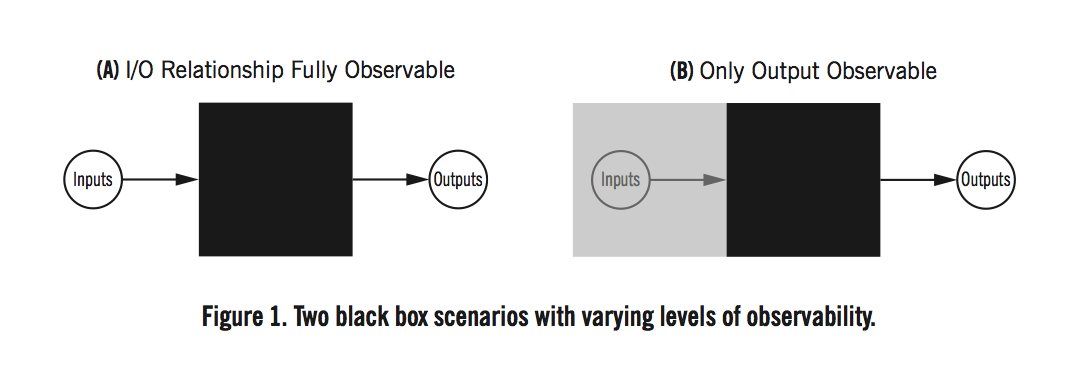
\includegraphics{images/BlackBoxObservability.png}
\caption{Figure 1. Two black box scenarios with varying levels of observability..}
\end{figure}

Figure 1 depicts two different black-box scenarios of interest to journalists reverse engineering algorithms by looking at the input-output relationship. The first scenario, in Figure 1(A), corresponds to an ability to fully observe all of an algorithm's inputs and outputs. This is the case for algorithms accessible via an online API, which facilitates sending different inputs to the algorithm and directly recording the output. 

Figure 1(B) depicts a scenario in which only the outputs of the algorithm are visible. The value-added model used in educational rankings of teachers is an example of this case. The teacher rankings themselves became available via a FOIA request, but the inputs to the algorithm used to rank teachers were still not observable. This is the most common case that data journalists encounter: A large dataset is available but there is limited (or no) information about how that data was transformed algorithmically. Interviews and document investigation are especially important here in order to understand what was fed into the algorithm, in terms of data, parameters, and ways in which the algorithm is used. It could be an interesting test of existing FOIA laws to examine the extent to which unobservable algorithmic inputs can be made visible through document or data requests for transparency. 

Sometimes inputs can be partially observable but not controllable; for instance, when an algorithm is being driven off public data but it's not clear exactly what aspect of that data serves as inputs into the algorithm. In general, the observability of the inputs and outputs is a limitation and challenge to the use of reverse engineering in practice. There are many algorithms that are not public facing, used behind an organizational barrier that makes them difficult to prod. In such cases, partial observability (e.g., of outputs) through FOIA, Web-scraping, or something like crowdsourcing can still lead to some interesting results. 

\chapter{Reverse Engineering: Practice }
In this subsection I detail five case studies of journalists using a reverse-engineering approach to understand algorithms. I'll draw on my experience analyzing censorship and defamation in search-engine autosuggest algorithms, as well as conversations I had with Michael Keller (The Daily Beast), Scott Klein (ProPublica), Jeremy Singer-Vine (Wall Street Journal), and Rob Barry (Wall Street Journal), all of whom have had direct experience working on or editing algorithmic accountability stories. The goal is to provide a summary of these efforts, to connect them to the theoretical component above, and to note the challenges encountered in employing the method in practice.

\section{Autocompletions on Google and Bing }
The Google autocomplete FAQ reads, ``We exclude a narrow class of search queries related to pornography, violence, hate speech, and copyright infringement.'' Bing, on the other hand, makes sure to ``filter spam'' as well as to ``detect adult or offensive content.'' Such editorial choices set the stage for broadly specifying the types of things that get censored. But what exactly are the boundaries of that censorship, and how do they differ among search engines? More importantly, what kinds of mistakes do these algorithms make in applying their editorial criteria? 

To answer these questions, I automatically gathered autosuggest results from hundreds of queries related to sex and violence in an effort to find those that were surprising or deviant.^{\href{#endnotes}{26}}Using a list of 110 sex-related keywords drawn from academic and slang sources as inputs to the algorithm, I looked to see which inputs resulted in zero output—suggesting a blocked word. While many of the most obvious words were outright blocked—like ``ass'' and ``tits''—a number of the search terms were not. The lack of blockage becomes more significant when adding the prefix ``child'' to the query, since some of the suggestions lead to child pornography, which is illegal and ought to be blocked. 

This case illustrates an ideal situation for the use of algorithmic-accountability reporting. Some transparency by the services through their FAQ's and blogs suggest a hypothesis and tip as to what types of input the algorithm might be sensitive to (i.e., pornography and violence-related words). Moreover, the algorithms themselves, both their inputs and outputs, are observable and accessible through APIs, which make it relatively easy to quickly collect a wide range of observations about the input-output relationship. 

\section{Autocorrections on the iPhone }
Another example of surfacing editorial criteria in algorithms comes from Michael Keller, now at Al Jazeera, but who at the time was working at The Daily Beast.^{\href{#endnotes}{27}}He dove into the iPhone spelling correction feature to see which words, like ``abortion'' or ``rape,'' the phone wouldn't correct if they were typed incorrectly. 

Michael's first attempt to sample this phenomenon was an API on the iPhone, which he used to identify words from a large dictionary that weren't getting corrected, essentially pruning down the space of inputs to see what the algorithm ``paid attention'' to. Eventually he noticed that some of the words the API did not correct were getting corrected when they were typed directly on an iPhone. There was a mismatch between what the API was reporting and what the user was experiencing. In order to mimic the real user experience he had to run an iPhone simulator on a number of computers, scripting it to act like a human typing in the word and then clicking the word to see if spelling corrections were presented. 

This example raises an important caveat. Sometimes algorithms expose inputs and make it possible to record outputs, but those outputs are then further transformed and edited before they get to the user interface. What really matters in the end is not just the output of the algorithm, but how that output is made available to the user. While this case is again an instance of full observability, it reminds us that we need to consider the output in context in order to understand and report on the algorithm's consequences. 

\section{Targeting Political Emails }
During the 2012 presidential campaign, Dan Sinker, head of the Knight- Mozilla OpenNews project, noticed that the Obama campaign was sending slight variations of the same email to different people. ProPublica picked up the tip and started gathering hundreds and then thousands of these targeted emails, soliciting them from people who were willing to forward them on to the news organization. Reporters had heard the Obama team was running a sophisticated data operation but no one inside the campaign was talking. 

The Message Machine,^{\href{#endnotes}{28}}as it came to be called, tried to reverse engineer how the campaign was using targeting information to adapt and personalize email messages for different recipients. In addition to collecting the emails, ProPublica solicited the recipients to fill out a survey asking about basic demographic information, where they lived, and if they had donated or volunteered for the campaign before. These survey answers then served as the input to the algorithm they were trying to dissect. In this case, the output was observable—crowdsourced from thousands of people—but the types of inputs used by the targeting algorithm were hidden behind the campaign wall and thus not controllable by journalists. Instead, ProPublica was tasked with determining, based on the outputs collected and a proxy for the inputs (collected with the survey), what types of inputs the campaign's targeting algorithm was actually paying attention to. 

In one instance the analysis was wrong, as Scott Klein, an editor who worked on Message Machine, explained to me. ``We slipped and we said that ‘in such and such an example they are targeting by age.''' After the campaign was over, however, Klein and his colleagues found that in fact the campaign was not targeting by age, but by another correlated variable: donation history. The lesson here for reverse engineering is that we need to be careful when using correlations to make claims about what inputs an algorithm is actually using. When we don't have access to the algorithm's inputs we can only make statistically informed guesses. Correlation does not imply causation, nor intent on the part of the designer. As much as algorithmic accountability can help us diagnose the existence of a problem, we have to go deeper and do reporting (when possible) to understand the motivations or intentions behind an algorithm. Ultimately, we still need to answer the question of ``why?'' 

\section{Price Discrimination in Online Commerce }
In 2013, the Wall Street Journal began probing e-commerce platforms to identify instances of potential price discrimination—the provision of different prices to different people.^{\href{#endnotes}{29}}By polling different websites it was able to spot several vendors, such as Staples, Home Depot, Rosetta Stone, and Orbitz, that were adjusting prices dynamically based on different factors like user geography, browser history, or mobile-browser use. In the case of Staples, it found that the input most strongly correlated to price was the distance to a rival's store, explaining about 90 percent of the pricing pattern. 

To get the story the WSJ had to simulate visiting the various sites from different computers and browsers in different geographies.^{\href{#endnotes}{30}}This initially required using various proxy servers that made it appear like the website was being loaded from different geographies. The publication's staff also created different archetype users and built user profiles using cookies to see how those user profiles might impact the prices recorded. This case again mimics Figure 1(A), wherein both inputs and outputs are fully observable. Yet, it was more complex than that of the autocomplete algorithm since a straightforward API wasn't available. Instead, the journalists had to painstakingly reconstruct profiles that simulated inputs to the algorithm, and look to see if any of the variables in those profiles led to significant differences in output (prices). 

Using reverse engineering on the scale of the Web surfaces several challenges, underscored both by the WSJ story and by academic efforts to reverse engineer personalization in Web search.^{\href{#endnotes}{31}}One of the issues is that sites like Staples might be using A/B testing to analyze whether or not subtle differences on their websites are useful to them. In other words, they're already running experiments on their sites, and to a reverse engineer it might look like noise, or just confusing irregularities. Algorithms may be unstable and change over time, or have randomness built in to them, which makes understanding patterns in their input-output relationship much more challenging. If you suspect the algorithm may be extremely dynamic and time-sensitive you may need to initiate all of your inputs to the algorithm in parallel in order to minimize the impact of a changing and dynamic algorithm. 

\section{Executive Stock Trading Plans }
Executives and corporate leaders sometimes use preset trading plans to avoid accusations of insider trading. The algorithmic plans can get triggered by any number of different parameters, like specific dates, stock prices, or announcements from competitors. The only catch is that the plans can't be based on inside information. When an executive makes a trade, he or she files a form with the SEC. The Wall Street Journal collected millions of these forms in an attempt to use reverse engineering to see if any of the plans were ``opportunistic''—if they appeared to be taking advantage of market timing to increase profits.^{\href{#endnotes}{32}}

In this case, the output was observable since the prices of all trades were known. What the WSJ was interested in was reverse engineering how timing information was being used by different plans as an input. Timing was observable, placing this scenario in Figure 1(A) where both inputs and outputs are known. Essentially the WSJ had a sampled input-output relationship for each executive's plan specified by the documents filed with the SEC. However, what it didn't know was any of the other inputs that could have also been feeding into these plans. Even though trade forms must be filed, the details of the plans themselves are hidden, leaving the reverse engineer to guess what inputs the algorithm was likely using. Perhaps competitor or sector prices are also inputs to some plans, requiring consideration of each variable in turn to assess whether there were correlations suggesting a connection. This case underscores the challenge with trying to understand which inputs an algorithm pays attention to. There is a huge space of potential inputs, some of which are observable and some of which are not. Practically speaking you have to choose which inputs you want to investigate to see if they are relevant to the algorithm. 

\chapter{Toward a Methodology }
Given the cases presented in the last section, as well as other examples of reverse engineering algorithms published in academic or non-mainstream outlets,^{\href{#endnotes}{33,34,35,36,37}} there are several key challenges to launching an investigation into an algorithm: identifying a meaningful target, sampling the algorithm, and finding the story.

\section{Identification}
In looking for algorithms that we want to hold accountable, we might ask several questions: What are the consequences and impact of that algorithm for the public, how significant are those consequences, and how many people might be affected by or perceive an effect by the algorithm? We might ask whether the algorithm has the potential for discrimination, or whether errors made by the algorithm may create risks that negatively impact the public. When a classification decision has negative consequences, then looking for false positives, like Content ID's identifying fair-use content as infringing, can be a tip indicating a deeper story. We might also wonder about censorship: How might the algorithm steer public attention and filter information in meaningful patterns? 

Essentially what we're looking to identify is an algorithm that's made a bad decision, that somehow breaks an expectation for how we think it ought to be operating. Is the algorithm's output consistent with what we think it should be? And if not, what's driving that inconsistency—a bug, an incidental programming decision, or a deep seated design intent? Observations, tips, and digging through data are all ways that we can identify interesting and significant algorithmic decisions that might warrant accountability reporting.

\section{Sampling }
After choosing an algorithm on which to focus, the challenge then becomes how to sample the input-output relationship of the algorithm in some meaningful way. As indicated in the last section, there are many scenarios with varying degrees of observability as related to algorithmic inputs and outputs. Sometimes everything is out in the open and there are APIs that can be sampled, whereas other times inputs are obfuscated. Figuring out how to observe or simulate those inputs is a key part of a practical investigation involving reverse engineering. Reporting techniques and talking to sources are two ways to try to understand what inputs are being fed into an algorithm, but when trade secrets obscure the process we're often reduced to guessing (e.g., ``Targeting Political Emails'' and ``Executive Stock Trading Plans''). Figuring out what the algorithm pays attention to input-wise becomes as intriguing a question as how the algorithm transforms input into output. 

Given a potentially infinite sampling space, we must define what is interesting and important for us to feed into an algorithm. For my story on search-engine autocompletions I wanted to know which sex-related words were blocked by Google and Bing, as well as whether adding ``child'' to the query led to any difference in output; were child sex-related queries leading to child pornography as well? The sampling strategy followed from these questions. I constructed a list of 110 sex-related words drawn from both academic linguists and Urban Dictionary slang to act as the basis for queries. Of course there are many other words and permutations of query templates that I might have used—the richness of language and diversity of expression mean that it will always be hard to come up with the ``right'' queries when working with algorithms that deal in human language. 

Similarly, for Jeremy Singer-Vine working on the price discrimination story at the WSJ, an initial hurdle for the project was getting a representative sample from enough different and dispersed geographies. There are proxy servers that you can rent in different zip codes to do this, but they're not available in every area, nor are they often in the same zip codes as residential neighborhoods. Deciding how to sample the input-output relationship of an algorithm is the first key challenge, and a difficult dance between what you can sample and what you would like to sample in order to answer your question. 

Of course it's not just about getting any valid sample either. You also have to make sure that the sample simulates the reality of importance to your audience. This was a key difficulty for Michael Keller's project on iPhone autocorrections, which eventually demanded he simulate the iPhone with scripts that mimic how a human uses the phone. I had a similar experience using an API to do my analysis of Google and Bing autocompletions— the API results don't perfectly line up with what the user experiences. For instance, the Google API returns 20 results, but only shows four or 10 in the user interface (UI) depending on how preferences are set. The Bing API returns 12 results but only shows eight in the UI. Data returned from the API that never appears in the UI is less significant since users will never encounter it in their daily usage—so I didn't report on it even though I had it collected. 

In some cases, someone else has already done the sampling of an algorithm and left you with a large dataset that might represent some input-output relationship. Or you may not have any control of inputs because those inputs are actually individual people you're unable or not ethically willing to simulate, such as in ProPublica's Message Machine. Though observation of such data can still be useful, I would argue that an experimental methodology is more powerful as it allows you to directly sample the input-output relationship in ways that let you assess particular questions you may have about how the algorithm is functioning. Indeed, there is a strong connection between the reverse engineering I'm espousing here and the scientific method. Some computer scientists have even called computing ``the fourth great scientific domain'' (after physical, biological, and social domains) due to the sheer complexity of the artificial computing systems humankind has built, so big that their understanding demands study in the same ways as other natural disciplines.^{\href{#endnotes}{38}}

\section{Finding the story }
Once you've got the input-output relationship of your black box mapped out, the next step is to search and filter for newsworthy insights. In some sense this goes back to expectations that define whether the algorithm is missing the mark somehow, or is exhibiting some behavior that has implications for the audience. These expectations could be statistically based, built on an understanding of social and legal norms, or defined by comparing similar vendors of the technology like Google and Bing autocompletions, or iPhone and Android autocorrections. It can be useful to look at the false positives and false negatives for ideas about how and where the algorithm is failing. 

At the WSJ the first filter used for narrowing-in on e-commerce sites was a statistical one: the variance of prices returned from a site for a given item across a variety of geographies. If any non-random variance was observed, the site was marked for a more rigorous and in-depth analysis. Similarly, Rob Barry, who worked on the executive trading plans story for the WSJ, described to me a sophisticated data-mining technique involving clustering and Monte Carlo simulation to find newsworthy cases by trying to identify trading plans that fell outside of the norms of expectation. 
In my own projects I have used social and legal norms to help zero-in on stories inside the collected data.^{\href{#endnotes}{39}}In the case of the autocomplete algorithms, both Google and Bing had publicly expressed a desire to filter suggestions relating to pornography. Taking that a step further, child pornography is indeed a violation of the legal code, so searching for instances of that became a starting point for filtering the data I had collected. Knowing where the algorithm violates the designers' expectations (e.g., it lets through child pornography when the stated intent is not to do so), or where it may have unintended side effects can both make for interesting stories. 

Another editorial criterion that Google uses in its autocomplete results relates to blocking violence. As part of my analysis I also queried the algorithm using 348 words from the Random House ``violent actions'' list to see whether Google was steering users toward knowledge of how to act violently. Since violence becomes a more interesting story if it's being suggested toward other people or living things I filtered my results against man-, woman-, person-, and animal-related word lists, essentially creating a newsworthiness filter. This sped up my ability to go through the results. Rather than reading through 14,000 results, I was reviewing fewer than 1,000. 

Still, even with newsworthiness filters helping to identify possible stories, it's absolutely essential to have reporters in the loop digging deeper. For every site that was flagged as a statistical hit, Singer-Vine's team did a much more comprehensive analysis, writing custom code to analyze each. ``There's an incredible role for traditional reporting to play in a story like that,'' said Singer-Vine. Knowing what makes something a story is perhaps less about a filter for statistical, social, or legal deviance than it is about understanding the context of the phenomenon, including historical, cultural, and social expectations related to the issue—all things with which traditional reporting and investigation can help. Sure it can be hard to get the companies running these algorithms to open up in detail about how their algorithms work, but reaching out for interviews can still be valuable. Even a trickle of information about the larger goals and objectives of the algorithms can help you better situate your reverse-engineering analysis. Understanding intent and motives is an important piece of the puzzle. In covering the redistricting story last year, Scott Klein, the news applications editor at ProPublica, considered using some computational means to detect gerrymandering, but quickly decided that, ``it [gerrymandering] is a motive, not a shape,'' which ultimately made traditional reporting techniques much more effective for investigating the story.

\chapter{Discussion }
Looking forward, we're faced with a number of challenges to actualizing algorithmic accountability in practice. Here I briefly touch on some of those challenges, including issues of human resources, legality, ethics, and the role that transparency might still effectively play. 

Developing the human resource to do algorithmic-accountability reporting will take dedicated efforts to teach the computational thinking, programming, and technical skills needed to make sense of algorithmic decisions. While there is growing awareness of more complex algorithms among data journalists, the number of computational journalists with the technical skills to do a deep investigation of algorithms is still rather limited. Teaming computationally literate reporters with tech-savvy computer scientists might be one method for doing more algorithmic accountability reporting. Another way would be to train journalists themselves in more computational techniques. Either way, we probably need more experience with the method before we can effectively teach it. ``There's no conventional or obvious approach to it. It's a lot of testing or trial and error, and it's hard to teach in any uniform way,'' noted Jeremy Singer-Vine. I also spoke to Chase Davis, an assistant editor at The New York Times and instructor at the Missouri School of Journalism, who concurred: ``Teaching it explicitly at this point might be difficult…a beat would be a stretch because there's no single unifying theme to it. It crosses a lot of boundaries in a way that standard data-driven journalism or CAR does.'' 

Legally speaking, the reverse engineering of commercial software does have some pitfalls. Other than the Digital Millennium Copyright Act (DMCA), there are no laws that directly prohibit or restrict reverse engineering, and even the DMCA has exemptions.^{\href{#endnotes}{40}}Software vendors do typically add anti-reverse engineering clauses to End User License Agreements (EULAs),^{\href{#endnotes}{41}}forcing the decision: Is it okay to breach such a contract if it gets you closer to the truth about the algorithm? Helen Nissenbaum, a professor at New York University, has suggested that laws might be in order to stipulate limits on Terms of Service to allow more room for individuals to negotiate their relationship with online entities.^{\href{#endnotes}{42}}Perhaps more problematic is a law like the Computer Fraud and Abuse Act (CFAA). ^{\href{#endnotes}{43}}Peter Ludlow recounts the story of Andrew Auernheimer, who wrote a script to collect private customer information that was inadvertently available on a public AT&T site.^{\href{#endnotes}{44}}Auernheimer was prosecuted under the CFAA and sentenced to 41 months in prison. Tread carefully here and seek qualified legal advice before attempting to reverse engineer algorithms or collect data from corporate or government entities. 

Besides the legality of reverse engineering corporate or government systems, there are other ethical questions that arise in the context of studying algorithms. In particular we need to ask ourselves about the possible ramifications or negative consequences of publishing details of how certain algorithms work. Would publishing such information negatively affect any individuals? More importantly, perhaps, is the issue of gaming brought up in the earlier section on transparency. Goodhart's law states, again, that once people know about a measure it's no longer a good one since they'll start trying to manipulate it. By publishing details of how an algorithm functions, specifically information about what inputs it pays attention to, how it uses various criteria in a ranking, or what criteria it uses to censor, how might that allow the algorithm to be manipulated or circumvented? And who stands to benefit from that manipulation? If publishing reverse-engineering information on how Google-search ranking works helps SEO black-hats get more spam information into our search results, then what did we really accomplish? The ethical principal of beneficence offers guidance here: Try to maximize anticipated benefits while minimizing possible risks of harm to the public. 

It may still be too early to develop standards on how entities creating and running algorithms might be more transparent about their technical systems, while respecting their right to trade secrets and their desire to mitigate gaming. Ultimately, we need to find a workable balancing point between trade secrets and transparency. Well-trodden transparency policies in other domains do offer some opportunity to reflect on how such policy might be adapted for algorithms.^{\href{#endnotes}{45}}For instance, targeted transparency policies always indicate the boundaries of disclosure, a contentious point as that boundary will dictate the limits of trade secret, and the degree of time and money invested by the algorithm creator in publishing the required transparency information. A policy would also need to indicate what factors or metrics of the algorithm would be disclosed, the frequency of their disclosure (e.g., daily, monthly, or real-time), and the vehicle for communicating that information (e.g., a separate document, or integrated into the algorithmic output in some way). 

The challenge to standardizing what should be disclosed about algorithms may come down to building consensus about what factors or metrics are both significant and acceptable. Frequency of disclosure, as well as communication vehicle, are important for adoption, but before we get there we need to know the informational content that might be disclosed. The questions at the beginning of the ``Algorithmic Accountability'' section form the basis for aspects of algorithms that we might consider here. This includes things like (1) the criteria used to prioritize, rank, emphasize, or editorialize things in the algorithm, including their definitions, operationalizations, and possibly even alternatives; (2) what data act as inputs to the algorithm— what it ``pays attention'' to, and what other parameters are used to initiate the algorithm; (3) the false positive and false negative rate of errors made in classification, including the rationale for how the balance point is set between those errors; (4) training data and its potential bias, including the evolution and dynamics of the algorithm as it learns from data; and (5) the definitions, operationalizations, or thresholds used by similarity or classification algorithms. To achieve a comprehensive public audit of an algorithm, we need to reach a consensus about which of these factors might be appropriate to make public, or semi-public (e.g., to an escrow third-party auditor). The hope is that as we develop more experience doing algorithmic accountability reporting the factors that are most significant to embed in a standardized algorithmic transparency policy will come into clearer focus. 

In the case of algorithms, where complexity reigns, and the computational literacy of the public may be limited, the role of professional and more sophisticated interpreters of transparency information will be essential. In the same way that business journalists contextualize and help the public understand the information produced through financial transparency of companies, journalists will also be needed to frame, contextualize, and explain the transparency information about algorithms. 

It's worth noting that as news organizations also come to employ algorithms in the shaping of the news they report, whether that be in finding new stories in massive datasets or presenting stories interactively, some of the same issues with transparency arise—news organizations are, after all, corporations that may have trade secrets to keep or systems to buttress from manipulation. But with the recent shift toward transparency as a core ideal of the journalistic enterprise,^{\href{#endnotes}{46}}tensions emerge between the ideal of transparency and the reality of algorithms. Chase Davis noted that one of the main challenges to building newsroom algorithms is providing a window for the reporter into how a particular algorithmic decision was made. It remains to be seen how news organizations will incorporate the evidence that algorithms or simulations provide with an epistemology and ethic that demands full transparency. Perhaps the public editor of the future will also play the role of algorithmic ombudsman. 

\chapter{Summary and Moving Forward }
We're now operating in a world where automated algorithms make impactful decisions that can and do amplify the power of business and government. I've argued in this paper that we need to do better in deciphering the contours of that power. As algorithms come to regulate society and perhaps even implement law directly,^{\href{#endnotes}{47}}we should proceed with caution and think carefully about how we choose to regulate them back.^{\href{#endnotes}{48}}Journalists might 
productively offer themselves as a check and balance on algorithmic power while the legislative regulation of algorithms takes shape over a longer time horizon. 
In this paper I've offered a basis for understanding algorithmic power in terms of the types of decisions algorithms make in prioritizing, classifying, associating, and filtering information. Understanding those wellsprings of algorithmic power suggests a number of diagnostic questions that further inform a more critical stance toward algorithms. Given the challenges to effectively employing transparency for algorithms, namely trade secrets, the consequences of manipulation, and the cognitive overhead of complexity, I propose that journalists might effectively engage with algorithms through a process of reverse engineering. By understanding the input-output relationships of an algorithm we can start to develop stories about how that algorithm operates. 
Sure, there are challenges here too: legal, ethical, and technical, but reverse engineering is another tactic for the tool belt—a technique that has already shown it can be useful at times. Next time you hear about software or an algorithm being used to help make a decision, you might get critical and start asking questions about how that software could be affecting outcomes. Try to FOIA it, try to understand whether you can reverse engineer it, and when you're finished, write up your method for how you got there. By method-sharing we'll expand our ability to replicate these types of stories, and, over time, perhaps even develop enough expertise to suggest standards for algorithmic transparency that acknowledge business concerns while still surfacing useful information for the public.


\chapter{Endnotes}

1 Segal, David. ``Mugged by a Mug Shot Online.'' The New York Times, October 5, 2013. \href{http://www. nytimes.com/2013/10/06/business/mugged-by-a-mug-shot-online.html}{http://www. nytimes.com/2013/10/06/business/mugged-by-a-mug-shot-online.html}}.\\
2 Schwartz, Barry. ``Google Launches Fix to Stop Mugshot Sites From Ranking: Google's MugShot Algorithm.'' Search Engine Land, October 7, 2013. \href{http://searchengineland.com/google-launches-fix-to-stop-mugshot-sites-from-ranking-googles-mugshot-algorithm-173672.}{http://searchengineland.com/google-launches-fix-to-stop-mugshot-sites-from-ranking-googles-mugshot-algorithm-173672.} \\
3 Lessig, Lawrence. ``Code is Law.'' Harvard Magazine, 1999. \href{http://harvardmagazine.com/2000/01/code-is-law-html}{http://harvardmagazine.com/2000/01/code-is-law-html} \\
4 Friedman, Batya and Helen Nissenbaum. ``Bias in Computer Systems.'' ACM Transactions on Information Systems, 14 (3), 1996. \\
5 \href{http://www.merriam-webster.com/dictionary/algorithm}{http://www.merriam-webster.com/dictionary/algorithm}. \\
6 Denning, Peter J. ``Computing is a Natural Science.'' Communications of the ACM (CACM), 50 (7). July, 2007. \\
7 Flowers, Michael. ``Beyond Open Data: The Data-Driven City.'' Beyond Transparency: Open Data and the Future of Civic Innovation, 2013. \href{http://beyondtransparency.org/chapters/part-4/beyond-open-data-the-data-driven-city/}{http://beyondtransparency.org/chapters/part-4/beyond-open-data-the-data-driven-city}. \\
8 Perry, Walter and Brian McInnis. Predictive Policing: The Role of Crime Forecasting in Law Enforcement Operations. Rand, 2013. \href{http://www.rand.org/pubs/research_reports/RR233.html}{http://www.rand.org/pubs/research_reports/RR233.html}. \\
9 Walker, Joseph. ``State Parole Boards Use Software to Decide Which Inmates to Release.'' Wall Street Journal, October 11, 2013. \href{http://online.wsj.com/news/articles/SB10001424052702304626104579121251595240852}{http://online.wsj.com/news/articles/SB10001424052702304626104579121251595240852}. \\
10 Kalhan, Anil. ``Immigration Policing and Federalism Through the Lens of Technology, Surveillance, and Privacy.'' Ohio State Law Journal, Vol. 74, 2013. \\
11 Otterman, Sharon. ``Court Says Teacher Rankings Should Be Public.'' The New York Times, August 25, 2011. \href{http://cityroom.blogs.nytimes.com/2011/08/25/court-says-teacher-rankings-should-be-public/}{http://cityroom.blogs.nytimes.com/2011/08/25/court-says-teacher-rankings-should-be-public/}. \\
12 ``How ContentID Works.'' \href{https://support.google.com/youtube/answer/2797370?hl=en}{https://support.google.com/youtube/answer/2797370?hl=en} 
13 Baio, Andy. ``Copyright Kings Are Judge, Jury, and Executioner on YouTube.'' Wired, February 29, 2012. \href{http://www.wired.com/business/2012/02/opinion-baiodmcayoutube/}{http://www.wired.com/business/2012/02/opinion-baiodmcayoutube/}. \\
14 Kraemer, Felicitas, Kees van Overveld, and Martin Peterson. ``Is there an ethics of algorithms?'' Ethics and Information Technology. 13 (3), 2011. \\
15 ``Outsmarting the Social Services Fraudster.'' IBM White Paper, 2013. \\
16 Pariser, Eli. The Filter Bubble: How the New Personalized Web Is Changing What We Read and How We Think. Penguin Press, 2011. \\
17 Hui, Li and Megha Rajagopalan. ``At Sina Weibo's censorship hub, China's Little Brothers cleanse online chatter.'' Reuters, September 11, 2013. \href{http://www.reuters.com/article/2013/09/12/us-china-internet-idUSBRE98A18Z20130912}{http://www.reuters.com/article/2013/09/12/us-china-internet-idUSBRE98A18Z20130912}. \\
18 Fung, Archon, Mary Graham, and David Weil. Full Disclosure: The Perils and Promise of Transparency. Cambridge University Press, 2009. \\
19 42 USC § 2000ee–3 - Federal agency data mining reporting. \href{http://www.law.cornell.edu/uscode/text/42/2000ee-3}{http://www.law.cornell.edu/uscode/text/42/2000ee-3}. \\
20 2012 Data Mining Report. Office of the Director of National Intelligence. \\
21 Pasquale, Frank. ``Restoring Transparency to Automated Authority.'' Journal on Telecommunications & High Technology Law, 9 (235), 2011. \\
22 Goodhart's Law. \href{http://en.wikipedia.org/wiki/Goodhart's_law}{http://en.wikipedia.org/wiki/Goodhart's_law}. \\
23 Eilam, Eldad. Reversing: Secrets of Reverse Engineering. Wiley, 2005. \\
24 Chikofsky, Elliot. ``Reverse engineering and design recovery: a taxonomy.'' IEEE Software, 7 (1), January, 1990. \\
25 Singh, Ramandeep. ``A Review of Reverse Engineering Theories and Tools.'' International Journal of Engineering Science Invention, 2 (1), January, 2013. \\
26 Diakopoulos, Nicholas. ``Sex, Violence, and Autocomplete Algorithms.'' Slate, August, 2013. \href{http://www.slate.com/articles/technology/future_tense/2013/08/words_banned_from_bing_and_google_s_autocomplete_algorithms.html}{http://www.slate.com/articles/technology/future_tense/2013/08/words_banned_from_bing_and_google_s_autocomplete_algorithms.html}.\\
27 Keller, Michael. ``The Apple ‘Kill List': What Your iPhone Doesn't Want You to Type.'' The Daily Beast, July, 2013.\href{http://www.thedailybeast.com/articles/2013/07/16/the-apple-kill-list-what-your-iphone-doesn-t-want-you-to-type.html}{http://www.thedailybeast.com/articles/2013/07/16/the-apple-kill-list-what-your-iphone-doesn-t-want-you-to-type.html}. \\
28 Larson, Jeff and Al Shaw. ``Message Machine: Reverse Engineering the 2012 Campaign.'' ProPublica, July, 2012. \href{http://projects.propublica.org/emails/}{http://projects.propublica.org/emails/}. \\
29 Valentino-DeVries, Jennifer, Jeremy Singer-Vine, and Ashkan Soltani. ``Websites Vary Prices, Deals Based on Users' Information.'' Wall Street Journal, December 24, 2012. \href{http://online.wsj.com/ article/SB10001424127887323777204578189391813881534.html#}{http://online.wsj.com/ article/SB10001424127887323777204578189391813881534.html#}. \\
30 Singer-Vine, Jeremy, Ashkan Soltani, and Jennifer Valentino-DeVries. ``How the Journal Tested Prices and Deals Online.'' Wall Street Journal, December 23, 2012. \href{http://blogs.wsj.com/ digits/2012/12/23/how-the-journal-tested-prices-and-deals-online/}{http://blogs.wsj.com/ digits/2012/12/23/how-the-journal-tested-prices-and-deals-online/}. \\
31 Hannak, Aniko, et al. ``Measuring Personalization of Web Search.'' Proceedings of the World Wide Web Conference (WWW), 2013. \\
32 Pulliam, Susan and Rob Barry. ``Executives' Good Luck in Trading Own Stock.'' Wall Street Journal, November 27, 2012. \href{http://online.wsj.com/news/articles/SB10000872396390444100404577641463 717344178}{http://online.wsj.com/news/articles/SB10000872396390444100404577641463 717344178}. \\
33 Sweeney, Latanya. ``Discrimination in Online Ad Delivery.'' Communications of the ACM, 56 (5), 2013. \\
34 Mukherjee, Arjun, et al. ``What Yelp Fake Review Filter Might Be Doing?'' Proceedings of the International Conference of Weblogs and Social Media (ICWSM), 2013. \\
35 Shirriff, Ken. ``How Hacker News Ranking Really Works: Scoring, Controversy, and Penalties.'' November 18, 2013. \href{http://www.righto.com/2013/11/how-hacker-news-ranking-really-works.html}{http://www.righto.com/2013/11/how-hacker-news-ranking-really-works.html}. \\
36 Guha, Saikat, et al. ``Challenges in Measuring Online Advertising Systems.'' Proc. Internet Measurement Conference (IMC), 2010. \\
37 Baker, Paul and Amanda Potts. ``‘Why do white people have thin lips?' Google and the perpetuation of stereotypes via auto-complete search forms.'' Critical Discourse Studies, 10 (2), 2013. \\
38 Rosenbloom, Paul. On Computing: The Fourth Great Scientific Domain. MIT Press, 2013. \\
39 Diakopoulos, Nicholas. ``Algorithmic Defamation: The Case of the Shameless Autocomplete.'' Tow Center for Digital Journalism, Columbia University, August 6, 2013. \href{http://towcenter.org/blog/algorithmic-defamation-the-case-of-the-shameless-autocomplete/}{http://towcenter.org/blog/algorithmic-defamation-the-case-of-the-shameless-autocomplete/}. \\
40 \href{http://www.copyright.gov/1201/}{http://www.copyright.gov/1201/}. \\
41 Eilam, Eldad. Reversing: Secrets of Reverse Engineering. Wiley, 2005. \\
42 Nissenbaum, Helen. ``From Preemption to Circumvention: If Technology Regulates, Why Do We Need Regulation (and Vice Versa)?'' Berkeley Technology Law Journal, 26 (3), 2011. \\
18 USC § 1030 - ``Fraud and related activity in connection with computers.'' \href{http://www.law.cornell.edu/uscode/text/18/1030.}{http://www.law.cornell.edu/uscode/text/18/1030}\\
44 Ludlow, Peter. ``Hacktivists as Gadflies.'' The New York Times, April 13, 2013. \href{http://opinionator.blogs.nytimes.com/2013/04/13/hacktivists-as-gadflies/}{http://opinionator.blogs.nytimes.com/2013/04/13/hacktivists-as-gadflies/}.\\
45 Fung, Archon, Mary Graham, and David Weil. ``Full Disclosure: The Perils and Promise of Transparency''. Cambridge University Press, 2009.\\
46 McBride, Kelly and Tom Rosenstiel. ``The New Ethics of Journalism: Principles for the 21st Century''. CQ Press, 2013.\\
47 O’Reilly, Tim. ``Open Data and Algorithmic Regulation." Beyond Transparency: Open Data and the Future of Civic Innovation, 2013. \href{http://beyondtransparency.org/chapters/part-5/open-data-andalgorithmic-regulation/}{http://beyondtransparency.org/chapters/part-5/open-data-andalgorithmic-regulation/}.\\
48 Citron, Danielle Keats. ``Technological Due Process.'' Washington University Law Review.
Vol. 85, 2007.\\
